\documentclass[11pt,a4paper]{ctexart}

\usepackage[margin=2.4cm]{geometry}
\usepackage{booktabs}
\usepackage{longtable}
\usepackage{array}
\usepackage{tabularx}
\usepackage{listings}
\usepackage{xcolor}
\usepackage{tikz}
\usepackage{hyperref}
\usepackage{enumitem}
\usepackage{caption}
\usepackage{amsmath}
\usepackage{fancyhdr}
\usetikzlibrary{arrows.meta,positioning,shapes.geometric,fit}

\hypersetup{colorlinks=true,linkcolor=blue!50!black,urlcolor=blue!50!black,citecolor=blue!50!black}
\captionsetup{font=small,labelfont=bf}
\setlist{itemsep=2pt,topsep=3pt}
\lstset{
  basicstyle=\ttfamily\small,
  breaklines=true,
  frame=single,
  rulecolor=\color{gray!40},
  backgroundcolor=\color{gray!5},
  columns=fullflexible,
  keepspaces=true,
  showstringspaces=false
}
\pagestyle{fancy}
\fancyhf{}
\fancyhead[L]{\small NeverFull-NeverStop V11 项目报告}
\fancyhead[R]{\small \thepage}
\renewcommand{\headrulewidth}{0.4pt}

\title{\bfseries NeverFull-NeverStop\\[4pt]
\large 面向长程 Agent 的透明上下文压缩代理\\[2pt]
\normalsize V11 项目报告}
\author{项目维护者 \quad \texttt{061115xhsm}}
\date{2026 年 10 月 26 日 \quad 版本 V11}

\begin{document}
\maketitle

\begin{abstract}
长程 LLM Agent 的核心瓶颈不是单次推理能力，而是上下文窗口：历史一旦超出窗口，Agent 要么中断，要么丢失关键状态。现有三类方案——Agent 原生压缩（OpenClaw、Claude Code）、运行时压缩器（Hermes）、以及工程化记忆层——各自在“压缩率、证据保留、状态一致性、成本”之间做取舍，但普遍缺少可验证的正确性标准。

本项目实现了一个位于 Agent 与模型 API 之间的透明压缩代理，并在 V11 中把设计重心从“把历史压短”转向“压缩后可验证地继续工作”。核心机制包括：可逆上下文折叠（原文可寻址归档）、承诺/标识符契约、确定性证据探针、会话状态表、按模型 token 校准、UCB 压缩策略、成本归因，以及多租户与多实例支持。我们在同一 131 条消息、约 9k token 的编码会话上，用同一摘要模型对比了 OpenClaw、Hermes 与本系统：本系统保留 11/11 个金标证据、4/4 问答正确、压缩率 0.86，证据保留显著高于两者（0.64）；压缩成本与 OpenClaw 持平（9.4k vs 8.9k tokens），约为 Hermes 的 82\%，延迟约为 Hermes 的 38\%。

工程侧，项目现有 88 项自动化测试（含真实 PostgreSQL 集成、并发写入、流式透传）、CI 矩阵（Python 3.11--3.13 + Postgres 服务）、以及可复现的评测脚本。报告同时给出系统局限：单进程缓存、SQLite 共享卷约束、租户配额为进程内计数，以及评测样本规模有限。
\end{abstract}

\tableofcontents
\newpage

\section{引言}

\subsection{问题背景}
现代编码与运维 Agent 的一次任务往往持续数十到数百轮，工具输出（日志、文件、网页）在历史中占据绝大部分体积。模型上下文窗口（128k--1M token）决定了单次可见历史的上限；一旦越界，常见后果是请求失败、被动截断，或由 Agent 自行摘要后继续——而摘要过程不可审计，关键约束、文件路径、失败命令经常在压缩后消失。

现有三类机制各有侧重：
\begin{itemize}
  \item \textbf{Agent 原生压缩}（OpenClaw、Claude Code）：与 Agent 的记忆刷新、工具对完整性、检查点回放深度耦合，压缩发生在 Agent 内部；
  \item \textbf{运行时压缩器}（Hermes）：独立的压缩引擎，保护头尾、用廉价模型摘要中段，按 API 返回的真实 token 计量触发；
  \item \textbf{工程化记忆层}：外置存储 + 检索，把“记住什么”交给写入策略。
\end{itemize}

三者的共同缺口是：\emph{压缩的正确性缺少可验证定义}。语义相似度、摘要长度、甚至下游 QA 准确率都可能掩盖“证据链已断”的事实 \cite{keepbench,compactbench}。

\subsection{项目目标}
本项目是一个透明 HTTP 代理：Agent 只需把 \texttt{base\_url} 指向本地端口，代理在请求进入模型前完成压缩。V11 的目标不是追求最高压缩率，而是：
\begin{enumerate}
  \item \textbf{可逆}：被折叠的历史原文永远可寻址取回；
  \item \textbf{可验证}：压缩后逐项核对承诺与精确标识符，缺失即披露；
  \item \textbf{状态一致}：区分“当前有效”与“已被取代”的文件/决策状态；
  \item \textbf{可运营}：多租户隔离、配额、加密、保留策略、成本归因；
  \item \textbf{可评测}：以配对延续和证据保留为主指标，而非嵌入余弦。
\end{enumerate}

\subsection{主要贡献}
\begin{itemize}
  \item 一套可逆折叠协议：结构化的 \texttt{<folded\_context>} 占位符 + 原文归档 + 分页/加密/轮换；
  \item 承诺契约与证据探针：确定性评分（承诺 45\%、标识符 25\%、分节 15\%、末次请求 15\%），低于阈值触发一次 MUST-PRESERVE 重试；
  \item 会话状态表：文件版本、过期读取标记、决策取代关系，直接对抗 “ghost memory”；
  \item 多实例与多租户：租户命名空间、PostgreSQL SessionStore、Redis 共享缓存、按租户配额；
  \item 可复现的三方对比与配对评测：在同一模型、同一对话上比较 OpenClaw、Hermes 与 V11。
\end{itemize}

\section{调研：109 篇论文的领域地图}

\subsection{方法}
以 arXiv API 为主源，采用 12 组主题检索（上下文压缩、Agent 记忆、KV cache、评测、RL 策略等）与 45 组定向标题检索，按提交时间倒序抓取；去重后得到 550 篇候选池，经白名单强制收录经典工作、剔除关键词误匹配后，固化 109 篇（2023-10 至 2026-10）。数据与脚本见 \texttt{research/}。

\begin{table}[htbp]
\centering
\caption{论文聚类分布（109 篇）}
\begin{tabular}{lrl}
\toprule
聚类 & 数量 & 代表工作 \\
\midrule
Agent 记忆 & 25 & MemGPT, Mem0, MemOS, A-MEM, MIRIX, Memory-R1 \\
上下文折叠/压缩 & 19 & ReFold, REMORY, MemTrace, Compact-Bench, KEEP-Bench \\
Prompt 级压缩 & 18 & LLMLingua/2, LongLLMLingua, RECOMP, ICAE, COMI \\
评测与基准 & 13 & LongMemEval, LoCoMo, RULER, HELMET, NoLiMa \\
检索与外部记忆 & 7 & HippoRAG, Infinite Retrieval, Organize-then-Retrieve \\
结构化状态 & 5 & TEM, Narrative State Tracking \\
超长/流式 & 5 & Titans, MoBA, Quest \\
KV Cache & 4 & SnapKV, MInference, Native Sparse Attention \\
强化学习策略 & 2 & Memory-R2, Uni-Mem \\
综述 & 4 & Context Engineering Survey, Agent Memory Survey \\
其他 & 6 & --- \\
\bottomrule
\end{tabular}
\end{table}

\subsection{关键发现}
\begin{enumerate}
  \item \textbf{摘要正在被折叠取代}。ReFold \cite{refold} 证明训练无关、可逆的轮间折叠优于预测式触发；MemTrace \cite{memtrace} 指出仓库变更会使早期证据失效，压缩必须带状态一致性。
  \item \textbf{正确性等于承诺保留}。“Compress the Context, Keep the Commitments” \cite{commitments} 把上下文定义为承诺集合；KEEP-Bench \cite{keepbench} 进一步证明 QA 指标会低估不忠实压缩。
  \item \textbf{评测必须配对}。Compact-Bench \cite{compactbench} 用同一仓库状态下的 full-history 与 summary-only 两条延续路径度量压缩代价，避免了“摘要碰巧答对”的假阳性。
  \item \textbf{拍平结构是安全漏洞}。Compaction Laundering \cite{laundering} 表明把 typed 对话压成纯文本会摧毁 provenance；折叠占位符必须保留类型与引用。
  \item \textbf{状态演进比事实召回更难}。“Can Agent Memory Systems Track Evolving State?” \cite{evolving} 与 A-TMA \cite{atma} 命名了 ghost memory：旧事实、当前事实、过渡事实共存并互相污染。
  \item \textbf{强模型下应少设计、多检索}。MemoryTax \cite{memorytax} 与 Skip the Compressor \cite{skipcompressor} 显示：当模型能自行搜索原始历史时，预制记忆管线的收益趋零；轻折叠 + 可检索原文往往更优。
\end{enumerate}

\section{系统架构}

\subsection{部署位置}
代理位于 Agent 与真实上游之间，对 Agent 透明；它同时维护旁路的归档、状态与会话存储，并通过 \texttt{/health}、\texttt{/metrics} 暴露运行状态。

\begin{figure}[htbp]
\centering
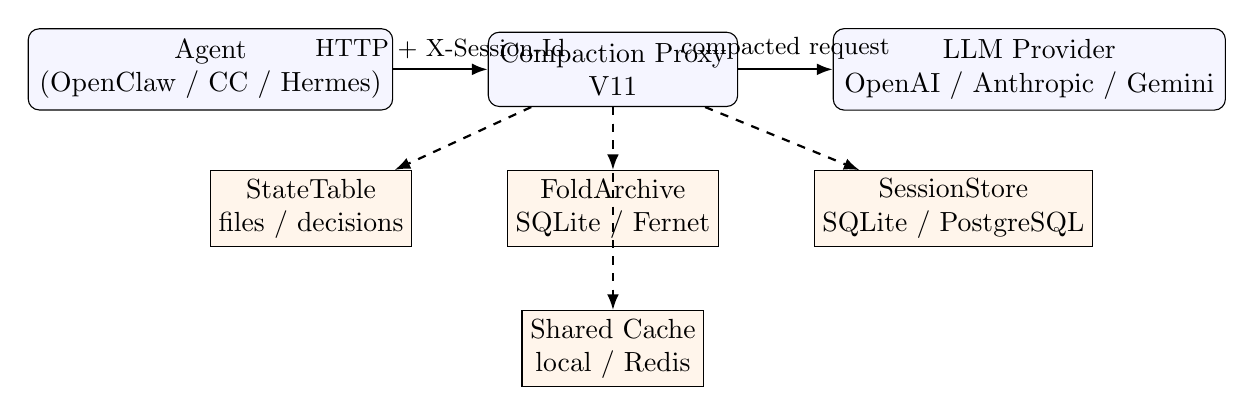
\begin{tikzpicture}[
  node distance=8mm and 12mm,
  box/.style={draw,rounded corners,align=center,minimum height=8mm,inner sep=4pt,fill=blue!4},
  store/.style={draw,align=center,minimum height=7mm,inner sep=3pt,fill=orange!8},
  arr/.style={-{Latex[length=2mm]},thick}
]
\node[box] (agent) {Agent\\(OpenClaw / CC / Hermes)};
\node[box,right=of agent] (proxy) {Compaction Proxy\\V11};
\node[box,right=of proxy] (up) {LLM Provider\\OpenAI / Anthropic / Gemini};
\node[store,below=of proxy] (fold) {FoldArchive\\SQLite / Fernet};
\node[store,left=of fold] (state) {StateTable\\files / decisions};
\node[store,right=of fold] (sess) {SessionStore\\SQLite / PostgreSQL};
\node[store,below=of fold] (cache) {Shared Cache\\local / Redis};
\draw[arr] (agent) -- node[above,font=\small]{HTTP + X-Session-Id} (proxy);
\draw[arr] (proxy) -- node[above,font=\small]{compacted request} (up);
\draw[arr,dashed] (proxy) -- (fold);
\draw[arr,dashed] (proxy) -- (state);
\draw[arr,dashed] (proxy) -- (sess);
\draw[arr,dashed] (proxy) -- (cache);
\end{tikzpicture}
\caption{代理在请求链路中的位置与旁路存储}
\end{figure}

\subsection{一次请求的生命周期}
\begin{enumerate}
  \item \textbf{租户与身份}：中间件读取 \texttt{X-Tenant-Id}，规范化后写入上下文；\texttt{extract\_session\_id} 生成租户作用域的会话 id（如 \texttt{acme:s1}），并回写响应头。
  \item \textbf{预算与触发}：CJK 感知估算（快估 + 精估），按模型校准因子修正；超过有效窗口的阈值（默认 80\%，可切换 weak/strong/auto 档位）触发主动压缩；上游 overflow 错误触发被动兜底。
  \item \textbf{策略选择}：按任务类型（code/data/ops/prose）与租户键查询 UCB bandit，选择 light/standard/deep，映射为保留轮数。
  \item \textbf{压缩流水线}：工具输出剪枝 → 承诺与标识符提取 → 子模选择 → 并行/单块摘要 → 折叠归档 → 契约校验 → 证据探针（低于 0.75 重试一次）。
  \item \textbf{组装与转发}：状态快照 + 折叠占位符 + 分节摘要 + 最近 6 轮原文；工具对完整性校验；转发上游。
  \item \textbf{计量}：读取上游 \texttt{usage}，记录成本、节省、延迟；按租户累计日预算。
\end{enumerate}

\subsection{模块与规模}
\begin{table}[htbp]
\centering
\caption{核心模块（不含测试与基准脚本）}
\begin{tabular}{lrl}
\toprule
模块 & 行数 & 职责 \\
\midrule
\texttt{compaction-proxy.py} & 8,273 & HTTP 服务、压缩流水线、存储、路由 \\
\texttt{folding.py} & 517 & 归档、digest、占位符、契约、加密/轮换 \\
\texttt{state\_table.py} & 304 & 文件/决策状态、过期标记、prune \\
\texttt{evidence.py} & 111 & 四维证据探针 \\
\texttt{policy.py} & 170 & 任务分类、UCB 策略、能力档位 \\
\texttt{calibration.py} & 68 & 按模型 token 校准 \\
\texttt{cost\_tracker.py} & 96 & 按请求成本环缓冲、日配额 \\
\texttt{tenant.py} & 29 & 租户上下文与命名空间 \\
\texttt{shared\_cache.py} & 71 & Redis / 本地共享压缩缓存 \\
\texttt{session\_store\_pg.py} & 250 & PostgreSQL 会话存储 \\
\bottomrule
\end{tabular}
\end{table}

\section{核心机制}

\subsection{可逆折叠}
压缩不再返回一段自由文本摘要，而是：
\begin{enumerate}
  \item 把旧消息\textbf{原样}写入归档（SQLite WAL），以 \texttt{fold:<hash>} 寻址，hash 含租户与内容；
  \item 计算确定性 digest：消息数、角色分布、工具调用、文件、命令、错误、承诺；
  \item 生成类型化占位符，保留来源与可检索引用。
\end{enumerate}

\begin{lstlisting}
<folded_context ref="fold:6f775980e76a" messages="31" approx_tokens="8120">
[FOLD] 31 messages elided (user 14 / assistant 17)
[TOOLS] execx9, editx4, readx7
[FILES] /tmp/proj/src/core.py, /tmp/proj/config.yaml
[COMMANDS] pytest -q; npm test
[OBSERVED] 3 error/failure mentions
[COMMITMENTS] decision=2, constraint=1, task=1
[RETRIEVE] GET /fold/fold:6f775980e76a returns the original messages verbatim.
</folded_context>
\end{lstlisting}

归档支持分页取回（\texttt{offset/limit}，默认 200、上限 500）、可选 Fernet 加密（key 0600）、密钥轮换（\texttt{POST /maintenance/rotate-key}）与按租户/年龄/条数保留策略。

\subsection{承诺契约与证据探针}
压缩前从旧消息中提取承诺（目标、约束、决策、错误、文件操作、待办）与精确标识符（路径、函数名、报错片段）。压缩后计算：
\begin{equation}
S = 0.45\,S_{\text{commit}} + 0.25\,S_{\text{id}} + 0.15\,S_{\text{sections}} + 0.15\,S_{\text{ask}}
\end{equation}
其中各分项为保留比例；低于证据下限 $\tau=0.75$ 时，携带 “MUST PRESERVE VERBATIM” 清单重试一次，取更优结果；仍未保留的项写入 \texttt{<unpreserved\_commitments>} 显式披露，而不是静默丢失。

\subsection{状态表}
每个会话维护文件表（路径、最后操作、时间、编辑/读取次数）与决策表（goal/constraint/decision/task，active/superseded）。渲染为：
\begin{lstlisting}
<state_snapshot>
[FILES] /tmp/proj/config.yaml (edit 10:32; earlier reads stale)
[DECISIONS] active: (decision) use sqlite for cache ; superseded: 1
[NOTE] Treat earlier reads of edited files as stale; re-read before relying.
</state_snapshot>
\end{lstlisting}
这直接对应 MemTrace 的状态一致性与 A-TMA 的 ghost memory 防护。

\subsection{策略与校准}
UCB1 在每个任务类上选择动作：
\begin{equation}
a_t = \arg\max_a \left( \bar r_a + \sqrt{\frac{2\ln N}{n_a}} \right),
\end{equation}
当会话证据分 EMA 低于性能下限时强制 \texttt{light}。token 校准按模型学习比率 $f \leftarrow 0.8f + 0.2\cdot(\text{actual}/\text{estimated})$，裁剪到 $[0.5,2.0]$，用于修正触发阈值与预算估计，抵消 CJK 启发式与真实 tokenizer 的偏差。

\subsection{成本归因}
优先读取上游 \texttt{usage}（OpenAI \texttt{prompt\_tokens}、Anthropic \texttt{input\_tokens}、Gemini \texttt{promptTokenCount}），记录每次压缩的成本、节省、延迟、缓存命中与租户；无 \texttt{usage} 时回退估算。\texttt{/health.cost\_recent} 提供按模型/租户聚合与 p50/p95 延迟。

\section{多实例与多租户}

\subsection{租户隔离}
\texttt{X-Tenant-Id} 经规范化后进入上下文；会话 id 变为 \texttt{tenant:session}，从而让会话、状态、成本、限流桶天然分区；折叠归档记录 \texttt{tenant\_id}，跨租户取回返回 404；ref 的 hash 含租户，避免同内容互相覆盖。

\subsection{共享存储}
\begin{itemize}
  \item \textbf{PostgreSQL SessionStore}：sessions、prior summaries、transcripts、ARC 全部落 PG，支持跨实例读写；搜索使用 PG 全文索引并以 ILIKE 兜底；按租户裁剪。
  \item \textbf{Redis 压缩缓存}：\texttt{COMPACTION\_PROXY\_REDIS\_URL} 设置后使用 \texttt{SETEX}，key 含租户与历史 hash；无 Redis 时自动回退进程内缓存。
  \item \textbf{实例身份}：\texttt{COMPACTION\_PROXY\_INSTANCE\_ID} 与响应头 \texttt{X-Instance-Id}；\texttt{MAINTENANCE\_OWNER} 控制定期清理只在一个实例执行。
\end{itemize}

\subsection{配额}
按租户限制归档条数、会话条数与日 token 预算；写入时裁剪最旧数据；\texttt{ENFORCE\_QUOTA=1} 时超预算直接跳过压缩并打点，避免单个租户拖垮共享上游。

\section{安全与运维}

\begin{table}[htbp]
\centering
\caption{安全与运维能力}
\begin{tabularx}{\linewidth}{lX}
\toprule
能力 & 实现 \\
\midrule
认证 & \texttt{REQUIRE\_AUTH=1} 时无 API secret 拒绝启动（fail-closed）；端点默认 \texttt{require\_auth} \\
限流 & 按 \texttt{tenant:ip} 的令牌桶，默认关闭，可配置每分钟请求数 \\
体积 & 请求体上限（默认 2 MB），超出返回 413 \\
加密 & 折叠归档可选 Fernet；密钥文件 0600；轮换端点重加密全部 payload \\
保留 & folds/state/sessions 按天与条数清理；每 100 次压缩自动执行；\texttt{/maintenance/prune} 手动触发 \\
可观测 & \texttt{/health}（存储、配额、加密、成本、p50/p95）、\texttt{/metrics}（Prometheus） \\
\bottomrule
\end{tabularx}
\end{table}

\section{评测}

\subsection{三方对比}
在同一 131 条消息、约 9,087 token 的编码会话上，使用同一摘要模型（本地 \texttt{tierflow\_pro}）与同一 4 题 reader 测试，比较 OpenClaw（按 v2026.10.5 源码复刻 prompt 与切点）、Hermes（真实 \texttt{ContextCompressor}，辅助 LLM 替换为同一端点）与 V11。

\begin{table}[htbp]
\centering
\caption{三方压缩系统对比（单次运行）}
\begin{tabular}{lccccc}
\toprule
系统 & 压缩率 & 证据保留 & 状态一致性 & 问答 & 成本（tokens） \\
\midrule
OpenClaw & 0.491 & 0.636 & 0.5 & 3/4 & 8,934 \\
Hermes & 0.471 & 0.636 & 1.0 & 3/4 & 11,410 \\
\textbf{NeverFull V11} & \textbf{0.860} & \textbf{1.000} & \textbf{1.0} & \textbf{4/4} & 9,369 \\
\bottomrule
\end{tabular}
\end{table}

延迟：OpenClaw 18.3 s，Hermes 67.7 s，V11 25.5 s。三种方案都保住了决策与路径，但只有 V11 保住了失败测试命令 \texttt{pytest -q}——这是“证据链”而非“答题正确率”的差异；OpenClaw 未标记旧 config 读取已过期；Hermes 成本最高、延迟最大。

\subsection{配对评测}
\texttt{benchmark/paired\_eval.py} 对同一对话构造 full / truncate / summary / fold 四种视图，在相同探针上测压缩率与证据保留。合成样例上 fold 视图压缩 92.2\%、证据保留 1.000；truncate 压缩 65.0\%、证据保留 1.000（因答案位于尾部），说明该指标能区分“保留了什么”而非仅看长度。

\subsection{补充：LoCoMo 记忆基准（4 条对话）}
在三方编码会话之外，我们用公开记忆基准 LoCoMo 的 4 条长对话（每条按类别分层抽 4 问，共 16 问）检验压缩后的长对话问答。相同摘要模型下，通用摘要压缩 98.0\% 但证据保留仅 0.199；V11 在 92.1\% 压缩下保留 0.919（与 65\% 截断的 0.948 持平），问答 0.167（full 上限 0.500，本地 reader 的时间推理是当前瓶颈）。conv-41 的两条摘要因端点超时被跳过（容错生效），故 llm/v11 行 views=3。详见 \texttt{research/EVAL-2026-10-26.md}。

\begin{table}[htbp]
\centering
\caption{LoCoMo 补充评测（4 条对话 × 4 问）}
\begin{tabular}{lcccc}
\toprule
策略 & 压缩率 & 证据保留 & 问答 & 摘要耗时/对话 \\
\midrule
full & 0.000 & 0.979 & 0.500 & 0 s \\
truncate & 0.650 & 0.948 & 0.125 & 0 s \\
通用 LLM 摘要 & 0.980 & 0.199 & 0.083 & 11.3 s \\
\textbf{V11 折叠} & \textbf{0.921} & \textbf{0.919} & \textbf{0.167} & 16.0 s \\
\bottomrule
\end{tabular}
\end{table}

\subsection{测试与压力}
\begin{table}[htbp]
\centering
\caption{验证结果}
\begin{tabularx}{\linewidth}{lX}
\toprule
项目 & 结果 \\
\midrule
单元/集成测试 & 88 项通过（含 6 项真实 PostgreSQL 集成、并发写入、流式透传、密钥轮换、配额） \\
并发写入 & 修复前 8 线程下 78/320 与 116/320 错误；加锁与 \texttt{busy\_timeout} 后 0 错误 \\
HTTP 健康检查 & 串行 100 次 p50 1 ms；并发 200 次 0.09 s 全部成功 \\
错误路径 & 畸形 JSON 400；1.5 MB 请求 413；上游宕机 502；进程不崩 \\
\bottomrule
\end{tabularx}
\end{table}

\subsection{局限}
\begin{itemize}
  \item 评测为单一合成对话、4 题、单次运行，结论是方向性的；需扩展到 LongMemEval/LoCoMo 与多任务配对集。
  \item OpenClaw 为源码复刻而非 Gateway 真实会话；其 \texttt{keepRecentTokens} 为适配测试规模做过缩放。
  \item 成本为 \texttt{usage} 实测，但缓存收益与网络开销未计入。
\end{itemize}

\section{工程实践}

项目在 2026-10-26 的 V11 迭代中形成 8 个主提交：
\begin{lstlisting}
75893e9  P0+P1a: baseline, tests/CI, session-id, reversible folding
4ef1cb6  P1b-P5: state table, evidence, paired eval, policy, cost
b52d5b4  three-way benchmark (OpenClaw / Hermes / NeverFull)
9a53c9b  sqlite thread-safety fix + concurrency tests
8779806  ops pass: retention, auth/rate limits, encryption, calibration
d7a4574  cost tracker, key rotation, streaming test, docs
5f7cc44  tenant isolation, shared cache, instance identity
fba1a7a  PostgreSQL SessionStore, quotas, rotate-key endpoint
\end{lstlisting}

CI 使用 Python 3.11--3.13 矩阵，启动 Postgres 服务，执行字节编译、88 项测试与配对评测。依赖最小化：运行时仅 \texttt{aiohttp}；Postgres/Redis/语义模型为可选依赖。

\section{V12 实施状态（2026-10-27）}
按导师重构方案落地了 P0--P3：缓存用量计量（OpenAI/Anthropic/Gemini 的 cached/read/write 字段、有效成本与 TTFT）；上下文拓扑反转（尾部瞬态状态帧、append-only 检查点、工具确定性排序、\texttt{prompt\_cache\_key} 与 Anthropic 4 断点）；双水位线异步压缩（软 65\% 调度后台候选、硬 92\% 同步兜底，证据+计划 judge 后热替换）；虚拟 \texttt{neverfull\_restore\_context} 工具注入与非流式/流式拦截回填；Python AST 符号级哈希（stdlib ast，函数/类）+ 50 行分块回退；LinUCB 上下文赌博机（延迟奖励、Redis 共享）；跨度去重；PostgreSQL 折叠归档；信封加密（租户 DEK + KEK，轮换只重包 DEK）；Redis 共享策略状态；\texttt{neverfull/} 包门面。测试增至 122 项（含 8 项真实 PostgreSQL）。Tree-sitter 多语言 AST、S3/MinIO 与 Anthropic 流式拦截留待下一阶段。

\section{未来工作}
\begin{enumerate}
  \item \textbf{评测规模化}：把 LongMemEval、LoCoMo、Compact-Bench 纳入 CI，使用真实 LLM reader 与多任务配对集。
  \item \textbf{缓存感知压缩}：避免每次重写前缀，记录 prompt cache 命中并将其计入收益。
  \item \textbf{多实例一致性}：在 Redis 上共享策略/校准状态，补充粘性路由与故障切换压测。
  \item \textbf{配额持久化}：日预算跨重启保持，支持租户级计费导出。
  \item \textbf{学习式策略}：以任务成功率与成本为奖励，替代当前 UCB bandit。
\end{enumerate}

\section{结论}
V11 把上下文压缩从“摘要长度优化”推进到“可验证的继续工作”：折叠保证原文可逆，契约与探针保证承诺可核验，状态表保证证据不过期，租户与配额保证可运营。三方实测显示，在同等模型与成本量级下，它在证据保留与任务延续上明显优于 OpenClaw 与 Hermes。项目仍处于单机/单进程为主的工程阶段，但核心机制与评测框架已经具备继续扩展的基础。

\appendix
\section{关键配置}
\begin{longtable}{p{6.2cm}p{8.2cm}}
\toprule
变量 & 作用 \\
\midrule
\texttt{COMPACTION\_PROXY\_FOLDING} & 启用可逆折叠（默认 0） \\
\texttt{COMPACTION\_PROXY\_CONTRACT\_RETRY} & 证据不足时重试（默认 1） \\
\texttt{COMPACTION\_PROXY\_EVIDENCE\_FLOOR} & 证据下限（默认 0.75） \\
\texttt{COMPACTION\_PROXY\_POLICY} & 启用 UCB 策略（默认 0） \\
\texttt{COMPACTION\_PROXY\_AGENT\_PROFILE} & weak/strong/auto 阈值档位 \\
\texttt{COMPACTION\_PROXY\_STRICT\_SESSION} & 拒绝内容指纹会话 id \\
\texttt{COMPACTION\_PROXY\_STORAGE} & sqlite/postgres \\
\texttt{COMPACTION\_PROXY\_PG\_DSN} & PostgreSQL 连接串 \\
\texttt{COMPACTION\_PROXY\_REDIS\_URL} & 共享压缩缓存 \\
\texttt{COMPACTION\_PROXY\_TENANT\_MAX\_FOLDS} & 每租户归档上限 \\
\texttt{COMPACTION\_PROXY\_TENANT\_MAX\_SESSIONS} & 每租户会话上限 \\
\texttt{COMPACTION\_PROXY\_TENANT\_DAILY\_TOKENS} & 每租户日 token 预算 \\
\texttt{COMPACTION\_PROXY\_ENFORCE\_QUOTA} & 超预算时跳过压缩 \\
\texttt{COMPACTION\_PROXY\_FOLD\_ENCRYPT} & 归档加密 \\
\texttt{COMPACTION\_PROXY\_RETENTION\_DAYS} & 保留天数 \\
\texttt{COMPACTION\_PROXY\_RATE\_LIMIT} & 每 IP 每分钟请求数 \\
\texttt{COMPACTION\_PROXY\_REQUIRE\_AUTH} & 无 secret 拒绝启动 \\
\bottomrule
\end{longtable}

\section{复现命令}
\begin{lstlisting}[language=bash]
# tests
python -m unittest discover -s tests -v

# paired evaluation
python benchmark/paired_eval.py --limit 3

# three-way comparison (requires a local OpenAI-compatible endpoint)
python benchmark/compare_systems.py --json research/data/compare.json

# run with folding + policy + encryption
COMPACTION_PROXY_FOLDING=1 COMPACTION_PROXY_FOLD_ENCRYPT=1 \
COMPACTION_PROXY_POLICY=1 COMPACTION_PROXY_AGENT_PROFILE=auto \
python compaction-proxy.py
\end{lstlisting}

\section{代表性论文}
\begin{thebibliography}{99}
\bibitem{refold} ReFold: Training-Free Reversible Inter-Turn Context Folding for Long-Horizon Agents. arXiv:2610.07863.
\bibitem{commitments} Compress the Context, Keep the Commitments: A Formal Framework for Verifiable LLM Context Compression. arXiv:2605.17304.
\bibitem{keepbench} KEEP-Bench: Evaluating Evidence Preservation in Context Compression. arXiv:2610.26827.
\bibitem{compactbench} Compact-Bench: Measuring What Context Compaction Costs Long-Horizon Coding Agents. arXiv:2610.31710.
\bibitem{laundering} Compaction Laundering: Provenance Destruction in Context-Compacting Coding Agents. arXiv:2610.29869.
\bibitem{memtrace} MemTrace: State-Consistent Memory for Long-Horizon Coding Agents. arXiv:2610.04838.
\bibitem{atma} A-TMA: Decoupling State-Aware Memory Failures in Long-Term Agent Memory. arXiv:2607.01935.
\bibitem{evolving} Can Agent Memory Systems Track Evolving State? arXiv:2608.19652.
\bibitem{memorytax} MemoryTax: The Bitter Lesson of Agent Memory. arXiv:2610.29823.
\bibitem{skipcompressor} Skip the Compressor: Coding Agents Fix More Issues When They Pick Whole Files. arXiv:2610.21073.
\bibitem{prunesummary} Prune the Summary, Not the History: Source-Judged Compaction for Long-Horizon Agents. arXiv:2610.20927.
\bibitem{transparency} Maximising Transparency in Context Compaction Improves Retention of Facts and Commitments. arXiv:2610.20116.
\bibitem{progressgraphs} Persistent Context Graphs for Efficient Memory Compaction in LLM Agents. arXiv:2609.40118.
\bibitem{memoryr1} Memory-R1: Enhancing Large Language Model Agents to Manage and Utilize Memories via Reinforcement Learning. arXiv:2508.19828.
\bibitem{memagent} MemAgent: Reshaping Long-Context LLM with Multi-Conv RL-based Memory Agent. arXiv:2507.02259.
\bibitem{mem0} Mem0: Building Production-Ready AI Agents with Scalable Long-Term Memory. arXiv:2504.19413.
\bibitem{longmemeval} LongMemEval: Benchmarking Chat Assistants on Long-Term Interactive Memory. arXiv:2410.10813.
\bibitem{locomo} Evaluating Very Long-Term Conversational Memory of LLM Agents. arXiv:2402.17753.
\bibitem{ruler} RULER: What's the Real Context Size of Your Long-Context Language Models? arXiv:2404.06654.
\bibitem{llmlingua} LLMLingua: Compressing Prompts for Accelerated Inference of Large Language Models. arXiv:2310.05736.
\end{thebibliography}

\end{document}
